\documentclass[11pt,]{article}
\usepackage[left=1in,top=1in,right=1in,bottom=1in]{geometry}
\newcommand*{\authorfont}{\fontfamily{phv}\selectfont}
\usepackage[]{mathpazo}


  \usepackage[T1]{fontenc}
  \usepackage[utf8]{inputenc}



\usepackage{abstract}
\renewcommand{\abstractname}{}    % clear the title
\renewcommand{\absnamepos}{empty} % originally center

\renewenvironment{abstract}
 {{%
    \setlength{\leftmargin}{0mm}
    \setlength{\rightmargin}{\leftmargin}%
  }%
  \relax}
 {\endlist}

\makeatletter
\def\@maketitle{%
  \newpage
%  \null
%  \vskip 2em%
%  \begin{center}%
  \let \footnote \thanks
    {\fontsize{18}{20}\selectfont\raggedright  \setlength{\parindent}{0pt} \@title \par}%
}
%\fi
\makeatother




\setcounter{secnumdepth}{0}

\usepackage{color}
\usepackage{fancyvrb}
\newcommand{\VerbBar}{|}
\newcommand{\VERB}{\Verb[commandchars=\\\{\}]}
\DefineVerbatimEnvironment{Highlighting}{Verbatim}{commandchars=\\\{\}}
% Add ',fontsize=\small' for more characters per line
\usepackage{framed}
\definecolor{shadecolor}{RGB}{248,248,248}
\newenvironment{Shaded}{\begin{snugshade}}{\end{snugshade}}
\newcommand{\KeywordTok}[1]{\textcolor[rgb]{0.13,0.29,0.53}{\textbf{#1}}}
\newcommand{\DataTypeTok}[1]{\textcolor[rgb]{0.13,0.29,0.53}{#1}}
\newcommand{\DecValTok}[1]{\textcolor[rgb]{0.00,0.00,0.81}{#1}}
\newcommand{\BaseNTok}[1]{\textcolor[rgb]{0.00,0.00,0.81}{#1}}
\newcommand{\FloatTok}[1]{\textcolor[rgb]{0.00,0.00,0.81}{#1}}
\newcommand{\ConstantTok}[1]{\textcolor[rgb]{0.00,0.00,0.00}{#1}}
\newcommand{\CharTok}[1]{\textcolor[rgb]{0.31,0.60,0.02}{#1}}
\newcommand{\SpecialCharTok}[1]{\textcolor[rgb]{0.00,0.00,0.00}{#1}}
\newcommand{\StringTok}[1]{\textcolor[rgb]{0.31,0.60,0.02}{#1}}
\newcommand{\VerbatimStringTok}[1]{\textcolor[rgb]{0.31,0.60,0.02}{#1}}
\newcommand{\SpecialStringTok}[1]{\textcolor[rgb]{0.31,0.60,0.02}{#1}}
\newcommand{\ImportTok}[1]{#1}
\newcommand{\CommentTok}[1]{\textcolor[rgb]{0.56,0.35,0.01}{\textit{#1}}}
\newcommand{\DocumentationTok}[1]{\textcolor[rgb]{0.56,0.35,0.01}{\textbf{\textit{#1}}}}
\newcommand{\AnnotationTok}[1]{\textcolor[rgb]{0.56,0.35,0.01}{\textbf{\textit{#1}}}}
\newcommand{\CommentVarTok}[1]{\textcolor[rgb]{0.56,0.35,0.01}{\textbf{\textit{#1}}}}
\newcommand{\OtherTok}[1]{\textcolor[rgb]{0.56,0.35,0.01}{#1}}
\newcommand{\FunctionTok}[1]{\textcolor[rgb]{0.00,0.00,0.00}{#1}}
\newcommand{\VariableTok}[1]{\textcolor[rgb]{0.00,0.00,0.00}{#1}}
\newcommand{\ControlFlowTok}[1]{\textcolor[rgb]{0.13,0.29,0.53}{\textbf{#1}}}
\newcommand{\OperatorTok}[1]{\textcolor[rgb]{0.81,0.36,0.00}{\textbf{#1}}}
\newcommand{\BuiltInTok}[1]{#1}
\newcommand{\ExtensionTok}[1]{#1}
\newcommand{\PreprocessorTok}[1]{\textcolor[rgb]{0.56,0.35,0.01}{\textit{#1}}}
\newcommand{\AttributeTok}[1]{\textcolor[rgb]{0.77,0.63,0.00}{#1}}
\newcommand{\RegionMarkerTok}[1]{#1}
\newcommand{\InformationTok}[1]{\textcolor[rgb]{0.56,0.35,0.01}{\textbf{\textit{#1}}}}
\newcommand{\WarningTok}[1]{\textcolor[rgb]{0.56,0.35,0.01}{\textbf{\textit{#1}}}}
\newcommand{\AlertTok}[1]{\textcolor[rgb]{0.94,0.16,0.16}{#1}}
\newcommand{\ErrorTok}[1]{\textcolor[rgb]{0.64,0.00,0.00}{\textbf{#1}}}
\newcommand{\NormalTok}[1]{#1}
\usepackage{longtable,booktabs}

\usepackage{graphicx,grffile}
\makeatletter
\def\maxwidth{\ifdim\Gin@nat@width>\linewidth\linewidth\else\Gin@nat@width\fi}
\def\maxheight{\ifdim\Gin@nat@height>\textheight\textheight\else\Gin@nat@height\fi}
\makeatother
% Scale images if necessary, so that they will not overflow the page
% margins by default, and it is still possible to overwrite the defaults
% using explicit options in \includegraphics[width, height, ...]{}
\setkeys{Gin}{width=\maxwidth,height=\maxheight,keepaspectratio}

\title{S01 - Operaciones Matriciales  }



\author{\Large Juan Carlos Martinez-Ovando\vspace{0.05in} \newline\normalsize\emph{ITAM}  }


\date{}

\usepackage{titlesec}

\titleformat*{\section}{\normalsize\bfseries}
\titleformat*{\subsection}{\normalsize\itshape}
\titleformat*{\subsubsection}{\normalsize\itshape}
\titleformat*{\paragraph}{\normalsize\itshape}
\titleformat*{\subparagraph}{\normalsize\itshape}


\usepackage{natbib}
\bibliographystyle{plainnat}
\usepackage[strings]{underscore} % protect underscores in most circumstances



\newtheorem{hypothesis}{Hypothesis}
\usepackage{setspace}

\makeatletter
\@ifpackageloaded{hyperref}{}{%
\ifxetex
  \PassOptionsToPackage{hyphens}{url}\usepackage[setpagesize=false, % page size defined by xetex
              unicode=false, % unicode breaks when used with xetex
              xetex]{hyperref}
\else
  \PassOptionsToPackage{hyphens}{url}\usepackage[unicode=true]{hyperref}
\fi
}

\@ifpackageloaded{color}{
    \PassOptionsToPackage{usenames,dvipsnames}{color}
}{%
    \usepackage[usenames,dvipsnames]{color}
}
\makeatother
\hypersetup{breaklinks=true,
            bookmarks=true,
            pdfauthor={Juan Carlos Martinez-Ovando (ITAM)},
             pdfkeywords = {Matrix algebra, linear operators, affine transformations.},  
            pdftitle={S01 - Operaciones Matriciales},
            colorlinks=true,
            citecolor=blue,
            urlcolor=blue,
            linkcolor=magenta,
            pdfborder={0 0 0}}
\urlstyle{same}  % don't use monospace font for urls

% set default figure placement to htbp
\makeatletter
\def\fps@figure{htbp}
\makeatother



% add tightlist ----------
\providecommand{\tightlist}{%
\setlength{\itemsep}{0pt}\setlength{\parskip}{0pt}}

\begin{document}
	
% \pagenumbering{arabic}% resets `page` counter to 1 
%
% \maketitle

{% \usefont{T1}{pnc}{m}{n}
\setlength{\parindent}{0pt}
\thispagestyle{plain}
{\fontsize{18}{20}\selectfont\raggedright 
\maketitle  % title \par  

}

{
   \vskip 13.5pt\relax \normalsize\fontsize{11}{12} 
\textbf{\authorfont Juan Carlos Martinez-Ovando} \hskip 15pt \emph{\small ITAM}   

}

}








\begin{abstract}

    \hbox{\vrule height .2pt width 39.14pc}

    \vskip 8.5pt % \small 

\noindent En esta sesion recordaremos algunas de las definiciones y operaciones
matriciales mas importantes empleadas en los metodos estadisticos
multivariados.


\vskip 8.5pt \noindent \emph{Keywords}: Matrix algebra, linear operators, affine transformations. \par

    \hbox{\vrule height .2pt width 39.14pc}



\end{abstract}


\vskip 6.5pt


\noindent  \subsection{Packages}\label{packages}

Emplearemos dos paquetes en \texttt{R} para ilustrar algunas de las
operaciones mas importantes de algebra matricial. En particular,
\texttt{VIGRA} es un paquete que implementa funciones en \texttt{c++}
para manipular matrices.

\begin{verbatim}
install.packages("VIGRA")
install.packages("OpenMx")
\end{verbatim}

\begin{center}\rule{0.5\linewidth}{\linethickness}\end{center}

\subsection{Racionalidad}\label{racionalidad}

Casi todos los modelos empleados en estadistica multivariada, machine
learning e, inclusive, deep learning, emplean representaciones
matriciales de los datos; ya sea respecto a los datos mismos o en
reducciones o resumenes de estos. Por ejemplo, si consideramos el
siguiente conjunto de datos,

\begin{Shaded}
\begin{Highlighting}[]
\NormalTok{data <-}\StringTok{ }\KeywordTok{read.csv}\NormalTok{(}\DataTypeTok{file =} \StringTok{"C:/Users/jcmo/Google Drive/Material.Cursos/EST46114/Sesiones/est46114/datos/EST46114_SSVS_Data.csv"}\NormalTok{, }
                 \DataTypeTok{header =} \OtherTok{TRUE}\NormalTok{, }\DataTypeTok{sep =} \StringTok{","}\NormalTok{)}
\NormalTok{data1 <-}\StringTok{ }\NormalTok{data[,}\KeywordTok{c}\NormalTok{(}\StringTok{"z1"}\NormalTok{,}\StringTok{"z2"}\NormalTok{,}\StringTok{"z3"}\NormalTok{)]}
\KeywordTok{plot}\NormalTok{(data1)}
\end{Highlighting}
\end{Shaded}

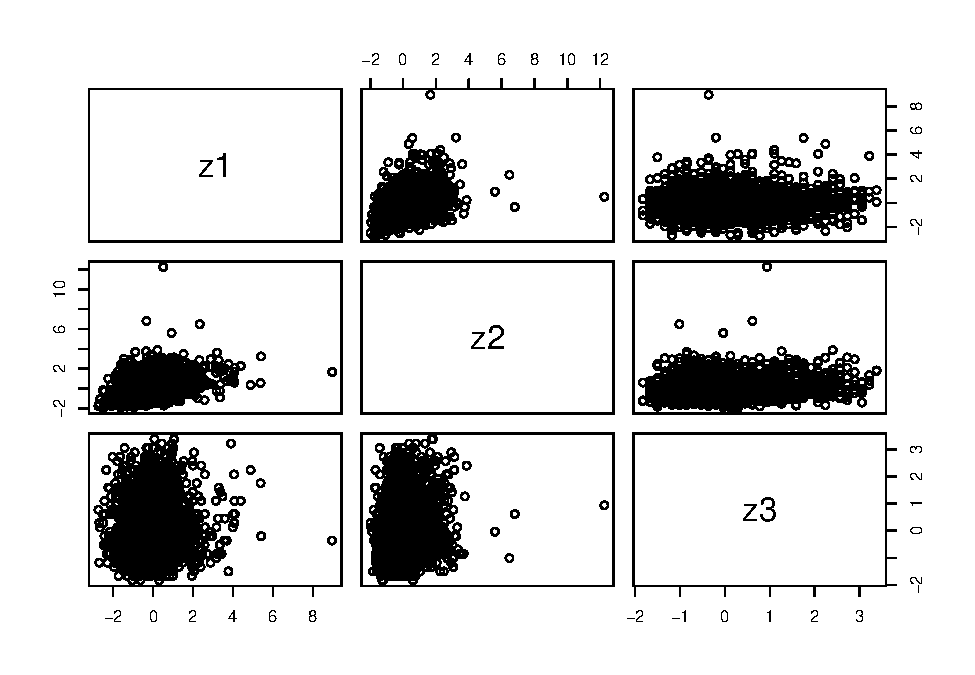
\includegraphics{est46114_s01_matrixops_svm_files/figure-latex/unnamed-chunk-1-1.pdf}

Algunas caracteristicas de estos datos son resumidos en la matriz de
varianzas y?o correlaciones,

\begin{Shaded}
\begin{Highlighting}[]
\NormalTok{correlaciones <-}\StringTok{ }\KeywordTok{cov}\NormalTok{(data1)}
\NormalTok{correlaciones}
\end{Highlighting}
\end{Shaded}

\begin{verbatim}
##            z1        z2         z3
## z1 1.00000000 0.3620867 0.03606888
## z2 0.36208673 1.0000000 0.19658670
## z3 0.03606888 0.1965867 1.00000000
\end{verbatim}

Note: En este caso las matrices coinciden pues los datos han sido
estandarizados.

La matriz de varianzas y covarianzas hace referencia al segundo momento
de los datos. Mas adelante veremos que algunas otras propiedades de
conjuntos de datos pueden resumirse en matrices de momentos de ordenes
mayores.

\subsection{Matrices}\label{matrices}

\subsubsection{Definiciones}\label{definiciones}

To understand your models you should understand matrices and linear
algebra. In some ways, OpenMx's USP or unique selling point is that it
is a matrix algebra processor. Most of the blog posts on this site cover
RAM-style modeling, but all of this sits on top of matrices:
\texttt{mxPath("A",\ "B")} simply inserts values into a matrix cell: Try
it and see!

\begin{Shaded}
\begin{Highlighting}[]
\KeywordTok{library}\NormalTok{(}\StringTok{"OpenMx"}\NormalTok{)}
\KeywordTok{data}\NormalTok{(demoOneFactor)}
\NormalTok{latents  =}\StringTok{ }\KeywordTok{c}\NormalTok{(}\StringTok{"G"}\NormalTok{)}
\NormalTok{manifests =}\StringTok{ }\KeywordTok{names}\NormalTok{(demoOneFactor)}
\NormalTok{m1 <-}\StringTok{ }\KeywordTok{umxRAM}\NormalTok{(}\StringTok{"One Factor"}\NormalTok{, }
             \DataTypeTok{data =} \KeywordTok{mxData}\NormalTok{(}\KeywordTok{cov}\NormalTok{(demoOneFactor), }
                           \DataTypeTok{type =} \StringTok{"cov"}\NormalTok{, }\DataTypeTok{numObs =} \DecValTok{500}\NormalTok{),}
    \KeywordTok{umxPath}\NormalTok{(latents, }\DataTypeTok{to =}\NormalTok{ manifests),}
    \KeywordTok{umxPath}\NormalTok{(}\DataTypeTok{var =}\NormalTok{ manifests),}
    \KeywordTok{umxPath}\NormalTok{(}\DataTypeTok{var =}\NormalTok{ latents, }\DataTypeTok{fixedAt =} \DecValTok{1}\NormalTok{)}
\NormalTok{)}
\KeywordTok{umx_show}\NormalTok{(m1)}
\end{Highlighting}
\end{Shaded}

Showing values for the S matrix:

\begin{longtable}[]{@{}lllllll@{}}
\toprule
& x1 & x2 & x3 & x4 & x5 & G\tabularnewline
\midrule
\endhead
x1 & 0.1 & . & . & . & . & .\tabularnewline
x2 & . & 0.15 & . & . & . & .\tabularnewline
x3 & . & . & 0.19 & . & . & .\tabularnewline
x4 & . & . & . & 0.27 & . & .\tabularnewline
x5 & . & . & . & . & 0.34 & .\tabularnewline
G & . & . & . & . & . & 1\tabularnewline
\bottomrule
\end{longtable}

So you should know about matrix algebra.

\subsubsection{What's a matrix?}\label{whats-a-matrix}

To quote \href{http://mathworld.wolfram.com/Matrix.html}{Wolfram} ``*A
matrix is a concise and useful way of uniquely representing and working
with linear transformations\ldots{} first formulated by Sylvester (1851)
and Cayley."

For our purposes, the benefit of matrices is their ability to represent
linear transformations and, in an optimiser, to allow us to solve
questions posed as linear algebra.

A matrix is a container or place from which something (else) originates.
Examples include the
\href{https://en.wikipedia.org/wiki/Extracellular_matrix}{extracellular
matrix}. In math, matrices consist of cells organized as rows and
columns, each cell of which can contain a number. The ``order'' of a
matrix is the number of rows followed by the number of columns. This a
matrix of order 3,2 looks like this:

\begin{verbatim}
|c1| c2 
\end{verbatim}

----\textbar{}---\textbar{}--- r1 \textbar{} . \textbar{} .\\
r2 \textbar{} . \textbar{} .\\
r3 \textbar{} . \textbar{} .

To begin to see the value of this representation, let's consider the
following 3 equations:

Y1 = a11 × b1 + a12 × b2

Y2 = a21 × b1 + a22 × b2

Y3 = a31 × b1 + a33 × b2

These can be re-expressed in 1-line of matrix algebra as:

\textbf{Y} = \textbf{a} × \textbf{b}

Where \textbf{Y} is a 3\emph{1 column matrix of the Y solutions,
\textbf{a} is a 3}2 matrix of values of \texttt{a}, and \textbf{b} is a
2*1 column matrix of \texttt{b} values.

Try it in R:

\begin{Shaded}
\begin{Highlighting}[]
\NormalTok{a =}\StringTok{ }\KeywordTok{matrix}\NormalTok{(}\KeywordTok{c}\NormalTok{(}\DecValTok{1}\NormalTok{, }\DecValTok{1}\NormalTok{, }\DecValTok{2}\NormalTok{, }\DecValTok{2}\NormalTok{, }\DecValTok{3}\NormalTok{, }\DecValTok{3}\NormalTok{), }\DecValTok{3}\NormalTok{ , }\DecValTok{2}\NormalTok{, }\DataTypeTok{byrow =} \OtherTok{TRUE}\NormalTok{)}
\NormalTok{b =}\StringTok{ }\KeywordTok{matrix}\NormalTok{(}\KeywordTok{c}\NormalTok{(.}\DecValTok{1}\NormalTok{, .}\DecValTok{2}\NormalTok{), }\DecValTok{2}\NormalTok{, }\DecValTok{1}\NormalTok{, }\DataTypeTok{byrow =} \OtherTok{TRUE}\NormalTok{)}
\NormalTok{Y =}\StringTok{ }\NormalTok{a }\OperatorTok\StringTok{ }\NormalTok{b; }
\KeywordTok{list}\NormalTok{(}\DataTypeTok{a =}\NormalTok{ a,}\DataTypeTok{b =}\NormalTok{ b, }\DataTypeTok{Y =}\NormalTok{ Y)}
\end{Highlighting}
\end{Shaded}

\url{http://stattrek.com/matrix-algebra/deviation-score.aspx?tutorial=matrix}

Matrix algebra is a tool for solving problems. Like all tools, it
represents or acts on things in a way that makes tasks easier to specify
or accomplish.

Matrix algebra makes the three core elements of SEM easier. These are

\begin{enumerate}
\def\labelenumi{\arabic{enumi}.}
\tightlist
\item
  Means
\item
  Covariances
\item
  Simultaneous equations
\end{enumerate}

Let's start trying to compute a mean.

To compute a mean, we want to sum all the elements of a column, and
divide them by nrows. Equivalently, we might multiply by 1/nrow

Let's compute the mean of each of three columns of a matrix of order
5,3.

\begin{Shaded}
\begin{Highlighting}[]
\NormalTok{n =}\StringTok{ }\DecValTok{5}
\NormalTok{myData <-}\StringTok{ }\KeywordTok{matrix}\NormalTok{(}\DataTypeTok{nrow =}\NormalTok{ n, }\DataTypeTok{byrow =} \OtherTok{TRUE}\NormalTok{, }\DataTypeTok{data =} \KeywordTok{c}\NormalTok{(}
\DecValTok{90}\NormalTok{, }\DecValTok{60}\NormalTok{, }\DecValTok{90}\NormalTok{, }
\DecValTok{90}\NormalTok{, }\DecValTok{90}\NormalTok{, }\DecValTok{28}\NormalTok{, }
\DecValTok{60}\NormalTok{, }\DecValTok{60}\NormalTok{, }\DecValTok{60}\NormalTok{, }
\DecValTok{60}\NormalTok{, }\DecValTok{60}\NormalTok{, }\DecValTok{90}\NormalTok{, }
\DecValTok{30}\NormalTok{, }\DecValTok{30}\NormalTok{, }\DecValTok{20}\NormalTok{))}
\NormalTok{myData}
\end{Highlighting}
\end{Shaded}

To form the means, we'll need the help of an n * 1 Identify matrix
(matrix of ones), let's call it \texttt{I}.

\begin{Shaded}
\begin{Highlighting}[]
\NormalTok{I =}\StringTok{ }\KeywordTok{matrix}\NormalTok{(}\DataTypeTok{data =} \DecValTok{1}\NormalTok{, }\DataTypeTok{nrow=}\NormalTok{ n, }\DataTypeTok{ncol =} \DecValTok{1}\NormalTok{)}
\end{Highlighting}
\end{Shaded}

Now if we pre-multiply the data by t(I), and then take the Kronecker
product of t(I) \%*\% I):

\begin{Shaded}
\begin{Highlighting}[]
\CommentTok{# means}
\KeywordTok{t}\NormalTok{(I) }\OperatorTok\StringTok{ }\NormalTok{myData }\OperatorTok\StringTok{ }\KeywordTok{solve}\NormalTok{(}\KeywordTok{t}\NormalTok{(I) }\OperatorTok\StringTok{ }\NormalTok{I)}
\end{Highlighting}
\end{Shaded}

We get the means

\begin{longtable}[]{@{}lll@{}}
\toprule
col 1 & col 2 & col 3\tabularnewline
\midrule
\endhead
66 & 60 & 57.6\tabularnewline
\bottomrule
\end{longtable}

\subsubsection{Computing a Covariance
matrix}\label{computing-a-covariance-matrix}

Covariances are simply the (sum of squared deviations from the mean)
divided by n or n-1.

Now we have the means, we can subtract these from each column to create
a column of leftovers: deviations from the mean.

And then devise a matrix formulation which sums the squares of these
deviations, returning a matrix of variances and covariances.

If we have n variables, we will want an n * n output matrix, containing
variances on the diagonal, and covariances on the off diagonal.

We first want not a row of means (like above) but a matrix with the
column mean in each cell. To get that, we do I times our row of means:

\begin{Shaded}
\begin{Highlighting}[]
\NormalTok{meanMyData =}\StringTok{ }\NormalTok{(I }\OperatorTok\StringTok{ }\NormalTok{(}\KeywordTok{t}\NormalTok{(I) }\OperatorTok\StringTok{ }\NormalTok{myData))}\OperatorTok{/}\NormalTok{n}
\end{Highlighting}
\end{Shaded}

Now we can subtract that from our data, to get a deviatio matrix:

\begin{Shaded}
\begin{Highlighting}[]
\NormalTok{devMatrix =}\StringTok{ }\NormalTok{myData }\OperatorTok{-}\StringTok{ }\NormalTok{meanMyData}
\end{Highlighting}
\end{Shaded}

The sum of squares of the deviations is t(dev) \%*\% dev

\begin{Shaded}
\begin{Highlighting}[]

\KeywordTok{t}\NormalTok{(devMatrix) }\OperatorTok\StringTok{ }\NormalTok{devMatrix}
\end{Highlighting}
\end{Shaded}

The covariance matrix is the sum-of-squares of the deviations divided by
n-1. We can check this by comparing it to R's built-in \texttt{cov()}
function:

\begin{Shaded}
\begin{Highlighting}[]

\NormalTok{ourCov =}\StringTok{ }\NormalTok{(}\KeywordTok{t}\NormalTok{(devMatrix) }\OperatorTok\StringTok{ }\NormalTok{devMatrix) }\OperatorTok{/}\StringTok{ }\NormalTok{(n}\OperatorTok{-}\DecValTok{1}\NormalTok{)}

\KeywordTok{cov}\NormalTok{(myData) }\OperatorTok{-}\StringTok{ }\NormalTok{ourCov}
\end{Highlighting}
\end{Shaded}

This is a nice chance too to mention that umx has a nifty quick-matrix
helper built in for rapidly building matrices:

\begin{Shaded}
\begin{Highlighting}[]

\NormalTok{A =}\StringTok{ }\KeywordTok{qm}\NormalTok{(}\DecValTok{0}\NormalTok{,}\DecValTok{1}\NormalTok{,}\DecValTok{2}\OperatorTok{|}
\DecValTok{3}\NormalTok{,}\DecValTok{4}\NormalTok{,}\DecValTok{5}\NormalTok{)}

\NormalTok{B =}\StringTok{ }\KeywordTok{qm}\NormalTok{(}
\DecValTok{6}\NormalTok{,}\DecValTok{7}\OperatorTok{|}
\DecValTok{8}\NormalTok{,}\DecValTok{9}\OperatorTok{|}
\DecValTok{10}\NormalTok{,}\DecValTok{11}\NormalTok{)}

\NormalTok{B }\OperatorTok\StringTok{ }\NormalTok{A}
    
\end{Highlighting}
\end{Shaded}

\section{\texorpdfstring{What's that ``pre- and post-multiply''
stuff?}{What's that pre- and post-multiply stuff?}}\label{whats-that-pre--and-post-multiply-stuff}

Often in
\href{https://en.wikipedia.org/wiki/Structural_equation_modeling}{SEM}
scripts you will see matrices being pre- and post-multiplied by some
other matrix. For instance, this figures in scripts computing the
\href{https://en.wikipedia.org/wiki/Genetic_correlation}{genetic
correlation} between variables. How does pre- and post-multiplying a
variance/covariance matrix give us a correlation matrix? And what is it
that we are multiplying this matrix by?

In general, a covariance matrix can be converted to a correlation matrix
by pre- and post-multiplying by a diagonal matrix with 1/SD for each
variable on the diagonal.

In R, \href{https://en.wikipedia.org/wiki/Invertible_matrix}{matrix
inversion} (usually signified by \textbf{A} -1) is done using the
\href{http://openmx.psyc.virginia.edu/wiki/matrix-operators-and-functions}{solve}()
function.

For the diagonal case, the inverse of a matrix is simply 1/x in each
cell.

\subsection{Example with variance matrix
A}\label{example-with-variance-matrix-a}

\begin{verbatim}
    A = matrix(nrow = 3, byrow = T,c(
        1,0,0,
        0,2,0,
        0,0,3)
    ); 

         [,1] [,2] [,3]
    [1,]    1    0    0
    [2,]    0    2    0
    [3,]    0    0    3

    invA = solve(A)

         [,1] [,2]  [,3]
    [1,]    1  0.0  0.00
    [2,]    0  0.5  0.00
    [3,]    0  0.0  0.33
\end{verbatim}

Any number times its inverse = 1. For Matrices
\texttt{solve(A)\ \%*\%\ A\ =\ I}.

\begin{verbatim}
invA %*% A #  = I = standardized diagonal
     [,1] [,2] [,3]
[1,]    1    0    0
[2,]    0    1    0
[3,]    0    0    1
\end{verbatim}

\subsubsection{An example with values (covariances) in the
off-diagonals}\label{an-example-with-values-covariances-in-the-off-diagonals}

\begin{Shaded}
\begin{Highlighting}[]
    
\NormalTok{A =}\StringTok{ }\KeywordTok{matrix}\NormalTok{(}\DataTypeTok{nrow =} \DecValTok{3}\NormalTok{, }\DataTypeTok{byrow =}\NormalTok{ T, }\KeywordTok{c}\NormalTok{(}
     \DecValTok{1}\NormalTok{, .}\DecValTok{5}\NormalTok{, .}\DecValTok{9}\NormalTok{,}
\NormalTok{    .}\DecValTok{5}\NormalTok{,  }\DecValTok{2}\NormalTok{, .}\DecValTok{4}\NormalTok{,}
\NormalTok{    .}\DecValTok{9}\NormalTok{, .}\DecValTok{4}\NormalTok{,  }\DecValTok{4}\NormalTok{)}
\NormalTok{);}

\NormalTok{I =}\StringTok{ }\KeywordTok{matrix}\NormalTok{(}\DataTypeTok{nrow =} \DecValTok{3}\NormalTok{, }\DataTypeTok{byrow =}\NormalTok{ T, }\KeywordTok{c}\NormalTok{(}
    \DecValTok{1}\NormalTok{,  }\DecValTok{0}\NormalTok{, }\DecValTok{0}\NormalTok{,}
    \DecValTok{0}\NormalTok{,  }\DecValTok{1}\NormalTok{, }\DecValTok{0}\NormalTok{,}
    \DecValTok{0}\NormalTok{,  }\DecValTok{0}\NormalTok{, }\DecValTok{1}\NormalTok{)}
\NormalTok{); }

\NormalTok{varianceA =}\StringTok{ }\NormalTok{I }\OperatorTok{*}\StringTok{ }\NormalTok{A }\CommentTok{# zero the off-diagonal (using regular multiplication, NOT matrix multiplication)}
\NormalTok{sdMatrix  =}\StringTok{ }\KeywordTok{sqrt}\NormalTok{(varianceA) }\CommentTok{# element sqrt to get SDs on diagonal (SD = sqrt(var) )}
\NormalTok{invSD     =}\StringTok{ }\KeywordTok{solve}\NormalTok{(sdMatrix) }\CommentTok{# 1/SD = inverse of sdMatrix}

\NormalTok{invSD}
\NormalTok{     [,}\DecValTok{1}\NormalTok{] [,}\DecValTok{2}\NormalTok{] [,}\DecValTok{3}\NormalTok{]}
\NormalTok{[}\DecValTok{1}\NormalTok{,]    }\DecValTok{1} \FloatTok{0.00}  \FloatTok{0.0}
\NormalTok{[}\DecValTok{2}\NormalTok{,]    }\DecValTok{0} \FloatTok{0.71}  \FloatTok{0.0}
\NormalTok{[}\DecValTok{3}\NormalTok{,]    }\DecValTok{0} \FloatTok{0.00}  \FloatTok{0.5}
\end{Highlighting}
\end{Shaded}

Any number times its inverse = 1, so this code sweeps covariances into
correlations

\begin{Shaded}
\begin{Highlighting}[]
\NormalTok{corr =}\StringTok{ }\NormalTok{invSD }\OperatorTok\StringTok{ }\NormalTok{A }\OperatorTok\StringTok{ }\NormalTok{invSD }\CommentTok{# pre- and post- multiply by 1/SD}
\KeywordTok{round}\NormalTok{(cor,}\DecValTok{2}\NormalTok{)}
\NormalTok{     [,}\DecValTok{1}\NormalTok{] [,}\DecValTok{2}\NormalTok{] [,}\DecValTok{3}\NormalTok{]}
\NormalTok{[}\DecValTok{1}\NormalTok{,] }\FloatTok{1.00} \FloatTok{0.35} \FloatTok{0.45}
\NormalTok{[}\DecValTok{2}\NormalTok{,] }\FloatTok{0.35} \FloatTok{1.00} \FloatTok{0.14}
\NormalTok{[}\DecValTok{3}\NormalTok{,] }\FloatTok{0.45} \FloatTok{0.14} \FloatTok{1.00}
\end{Highlighting}
\end{Shaded}

\subsection{Easy way of doing this in
R}\label{easy-way-of-doing-this-in-r}

Using diag to grab the diagonal and make a new one, and capitalising on
the fact that inv(X) = 1/x for a diagonal matrix

\begin{Shaded}
\begin{Highlighting}[]
\KeywordTok{diag}\NormalTok{(}\DecValTok{1}\OperatorTok{/}\KeywordTok{sqrt}\NormalTok{(}\KeywordTok{diag}\NormalTok{(A))) }\OperatorTok\StringTok{ }\NormalTok{A }\CommentTok{# note: The %&%  operator is short for pre- and post-mul}
\NormalTok{     [,}\DecValTok{1}\NormalTok{] [,}\DecValTok{2}\NormalTok{] [,}\DecValTok{3}\NormalTok{]}
\NormalTok{[}\DecValTok{1}\NormalTok{,] }\FloatTok{1.00} \FloatTok{0.35} \FloatTok{0.45}
\NormalTok{[}\DecValTok{2}\NormalTok{,] }\FloatTok{0.35} \FloatTok{1.00} \FloatTok{0.14}
\NormalTok{[}\DecValTok{3}\NormalTok{,] }\FloatTok{0.45} \FloatTok{0.14} \FloatTok{1.00}
\end{Highlighting}
\end{Shaded}

\subsection{Even-easier built-in way}\label{even-easier-built-in-way}

\begin{Shaded}
\begin{Highlighting}[]
\KeywordTok{cov2cor}\NormalTok{(A)}

\NormalTok{     [,}\DecValTok{1}\NormalTok{] [,}\DecValTok{2}\NormalTok{] [,}\DecValTok{3}\NormalTok{]}
\NormalTok{[}\DecValTok{1}\NormalTok{,] }\FloatTok{1.00} \FloatTok{0.35} \FloatTok{0.45}
\NormalTok{[}\DecValTok{2}\NormalTok{,] }\FloatTok{0.35} \FloatTok{1.00} \FloatTok{0.14}
\NormalTok{[}\DecValTok{3}\NormalTok{,] }\FloatTok{0.45} \FloatTok{0.14} \FloatTok{1.00}
\end{Highlighting}
\end{Shaded}




\newpage
\singlespacing 
\end{document}
